\chapter{Nasazení}

K testování a provozu webové aplikace jsem získál virtualizovaný server, ke kterému přistupuji pomocí SSH.

== pod carou ==
Program, který komunikuje zabezpečeným komunikačním protokolem. Používá TCP/IP.

\subsection{Virtuální privátní server}

Často se označuje zkratkou VSP. Bývá...

Výhodou je rychle nasazeni atd...
Nevýhodou sdílené prostředky s ostatními VPS.

% adresa na wiki https://cs.wikipedia.org/wiki/Virtu%C3%A1ln%C3%AD_priv%C3%A1tn%C3%AD_server

\section{Softwarové požadavky}

Aplikace běží na VPS s OS Ubuntu verze 15.10. Na veřejné adrese virtulního serveru
je dostupná RESTová webová služba Catcher, s níž může zvnějšku komunikovat libovolná aplikace,
která disponuje HTTP protokolem a dostupností běžného portu 80. Jako prostředník mezi klientskou aplikací
a uWSGI 2.0.12, jehož úkolem je udržovat Catchera, zde běží webový server Nginx 1.9.3.
Data se ukládají na databázový server MySQL verze 5.6.28.

Pro běh aplikace byly stáhnuty všechny potřebné balíčky včetně pipu, jenž slouží pro správu nesystémových knihoven v Pythonu. Detailní seznam všech zásvislostí obsahuje soubor README.md, uložený v rodičovském adresáři projektu. Lepší správu souborů mi pak zajistil program Midnight Commander.


SSH (Secure Shell) je v informatice označení pro program a zároveň pro zabezpečený komunikační protokol v počítačových sítích, které používají TCP/IP. SSH byl navržen jako náhrada za telnet a další nezabezpečené vzdálené shelly (rlogin, rsh apod.), které posílají heslo v nezabezpečené formě a umožňují tak jeho odposlechnutí při přenosu pomocí počítačové sítě.[1] Šifrování přenášených dat, které SSH poskytuje, slouží k zabezpečení dat při přenosu přes nedůvěryhodnou síť, jako je například Internet.

\begin{figure}[ht!]
\centering
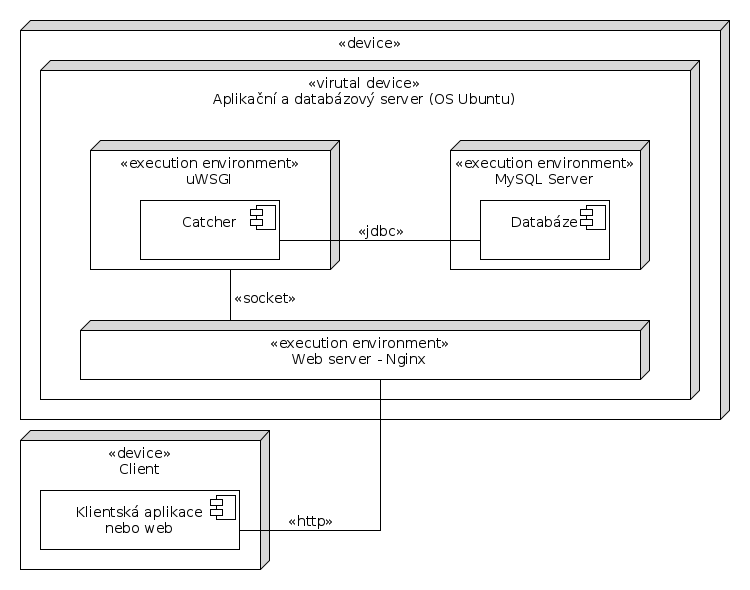
\includegraphics[width=130mm]{./images/diagram-nasazeni.png}
\caption{Diagram nasazení\label{overflow}}
\end{figure}

\section{uWSGI}

Aby bylo lépe pochopitelné zapojení uWSGI do celého procesu nasazení, popíšeme si jej trochu detailněji.

Projekt uWSGI je malý program, který se stará o management procesu aplikace. Funguje jako prostředník mezi aplikací a webovým serverem, se kterými komunikuje vlastním uwsgi protokolem, respektive standartním WSGI. Detaily komunikace jsou vidět na obrázku xxx.

% TODO: hezky diagram a povidani je na https://www.zdrojak.cz/clanky/produkcni-nasazeni-django-aplikaci-na-cherokee-pomoci-wsgi/ 

== pod carou ==
WSGI je komunikační protokol mezi aplikací napsanou v Pythonu a webovým serverem.

\subsection{uWSGI úloha}

Spuštění webové aplikace provadím následujícím příkazem:

uwsgi --socket localhost:8080 --wsgi-file ./restapi.py --callable api &

Proces poslouchá na portu 8080 a po celou dobu běží na pozadí.

\section{Konfigurace}

\subsection{Konfigurační soubor}

Protože všechny moje zdrojové kódy byly zveřejněny v repozitáři na GitHubu, nebylo správné aby obsahovaly jakkákoliv hesla. Pro tyto potřeby byl vytvořen konfigurační soubor, který mám zazálohavný na vlastním cloudovém uložišti a pomocí programu wget si jej stahuju do daného adresáře vždy, když je změněn. Tento konfigurační soubor obsahuje hesla k produkční a testovací databázi nebo k emailovému účtu, který používám pro obnovu hesla uživatelů.

\subsection{Databáze}

Pro přístup do databáze bylo potřeba vytvořit uživatele s právem zapisovat, číst a mazat.
Tento účet se nadále autentizuje heslem, které je uložené v konfiguračním souboru.

Příkazy pro vytvoření uživatele:

CREATE USER 'catcher-server'@'localhost' IDENTIFIED BY 'tajne_heslo';
GRANT SELECT, INSERT, UPDATE, DELETE ON catcher. * TO 'catcher-server'@'localhost';

\subsection{Nginx}

Protože disponuji pouze jednou veřejnou adresou na VPS, bylo potřeba webový server nakonfigurovat tak, aby dokázal obsluhovat požadavky webové aplikace i požadavky
na zobrazení dokumentace. Konfigurace na serveru byla následující:

\subsubsection*{/etc/nginx/sites-enabled/catcher.conf}

upstream catcher_uwsgi {
    server localhost:8080;                                          # adresa a port, na které přeposílám požadavky pro Catchera
}

server {
    listen       80;                                                # poslouchej na portu 80 na ipv4
    listen       [::]:80;                                           # poslouchej na portu 80 na ipv6
    server_name  catcher.zlutazimnice.cz *.catcher.zlutazimnice.cz; # jméno serveru
    charset      utf-8;
    index        index.html;

    client_max_body_size 75M;                                       # maximální velikost uploadu

    # dokumentace na catcher.zlutazimnice.cz
    location / {
        root   /var/www/catcher;                                    # adresář s obsahem webu
    }

    # webová aplikace na catcher.zlutazimnice.cz/api
    location /api {
        include     uwsgi_params;
        uwsgi_pass  catcher_uwsgi;                                  # upstream, pro spojení s uwsgi
    }
}

Pro vývoj jsem použil trochu odlišnou konfiguraci. V prvních fázích jsem dokonce ani Nginx používat nemusel, protože uWSGI umožňuje simulovat chování web serveru a jako prostředníka jsem jej tedy mohl vynechat. Pro produkční nasazení ale není tento postup doporučen.

\section{Údržba}

Standartem pro větší aplikace by měl být monitorovací systém, který sleduje zátěž jednotlivých komponent (webová aplikace, databáze, webový server atd.) a v případě výpadku informuje administrátora sms zprávou nebo emailem. Catcher však disponuje vlastností, že ještě nějakou dobu nebude nasazen do ostrého provozu a pro tyto potřeby by měl stačit cron, který by v pravidelných intervalech oťukával aplikaci a určil, zda běží. Kromě toho cron může pravidelně zálohovat databázi příkazem dump. V případě výpadku by tak stačilo aplikaci opravit a nahrát poslední zálohu.

Catcher aktuálně disponuje pouze manuálním zálohováním databáze.

== pod carou ==
Jde o softwarového démona, který slouží k automatickému spouštění periodicky se opakujících příkazů a procesů.

\section{Co by šlo udělat lépe}

Během vývoje jsem se setkal se zajímavými nástroji, na které v tomto projektu nezbyla kapacita. Jejih použití by přineslo několik zlepšení, proto jsem se rozhodl je zde uvést:

%list:

Virtualenv, Codevoc, Travis CI

% TODO: IDEA: Lze se zminit o testovani a prubezne integraci. Napriklad napsat, ze mame zajem v budoucnu pouzivat Codevoc (mozna spis testovani) nebo Travis CI.